%!TEX root = bioPrediction_main.tex
% \section{Analysis and Results}

% \begin{table*}[h]
%   \centering
%   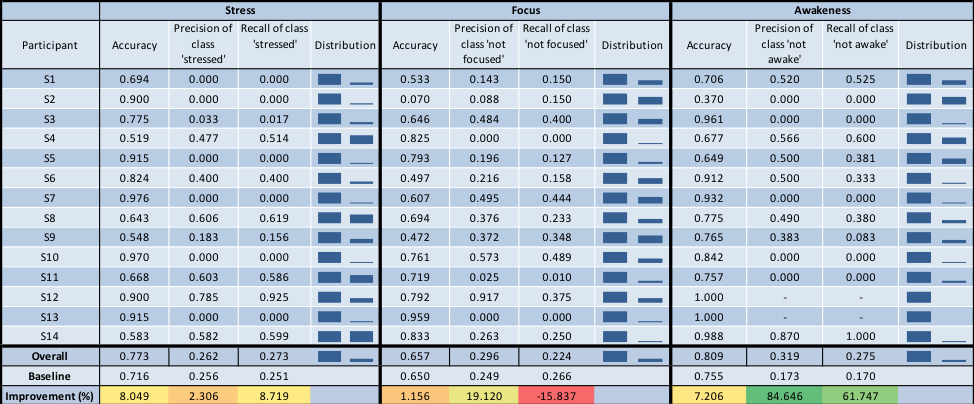
\includegraphics[width=1.0\textwidth]{rq1performance.png}
%   \caption{Results of leave one out evaluation on individual models. The overall and baseline rows contain weighted averages of the individual models, to account for the large imbalance in the data collected
%   }
%    \label{rq1performance}
% \end{table*}

% To evaluate the ability of predicting a knowledge worker's stress, focus, and awakeness in the workplace, we trained and tested machine learning classifiers using a leave-one-out cross validation. In particular, we used the features extracted from the collected data as the input data and binarized the participants' experience samples on stress, focus and awakeness into two classes each (e.g., 'stressed' and 'not stressed'). 

% % random forest best
% In a first step, we compared multiple classifiers using the popular machine learning library scikit-learn \todo{add ref back in} and performing a grid search analysis to determine the optimal hyperparameters for each classifier. Our analysis showed that random forest outperfoms all other classifiers, including Naive Bayes, decision trees, support vector machine, random forest, and a multilayer perceptron neural network. The optimal values for random forest and the three output measures are listed in Table \todo{fill table below (see comment for values)}. For the remainder of this paper, we will be referring to random forest classifiers trained with these hyperparameters.\\[-0.1cm]
% % for stress they were (minimum samples for split = 4, # of estimators = 100, max features = 0.5, k=300), for focus they were (minimum samples for split = 4, # of estimators = 50, max features = 0.5, k=200), and for awakeness they were (minimum samples for split = 4, # of estimators = 100, max features = 0.25, k=800)

% \begin{table}[H]
% 	\begin{centering}
%     \begin{tabular}{llll}
%       \hline
%       Variable & K & Number of 		Estimators & Minimum Samples to Split \\
%       \hline
%     \end{tabular}
%     \end{centering}
% \end{table}

% \subsection{Predicting Stress, Focus \& Awakeness} \label{secOverallAccuracy}

% Since peoples experience of stress, focus and awakeness as well as their physiological manifestation can vary a lot~\cite{}\todo{find good references here, including https://pdfs.semanticscholar.org/d17d/930333da55860189205707252eef6be6c663.pdf}, we trained individual classifiers for each participant. The results of our analysis are reported in Table~\ref{rq1performance}. For our analysis, we report values of accuracy, one of the most commonly used metric to compare performance, as well as precision and recall of the classes of interest: 'stressed', 'not focused', and 'not awake'. Since the imbalance in the data can lead to high accuracy values if a classifier always just predicts the more likely class while ignoring the class of higher importance and interest, precision and recall of the class of interest can be more adequate metrics in this case~\cite{yap2014,bhattacharyya_data_2011}\todo{also cite: https://pdfs.semanticscholar.org/d17d/930333da55860189205707252eef6be6c663.pdf}. 
% % However, the imbalance in the data can lead to a classifier with high accuracy if it always just predicts the more likely class while ignoring the class of higher importance and interest in our case (i.e. stressed, not focused, not awake). Therefore, we further report the precision and recall for the three classes 'stressed', 'not focused' and 'not awake'. 


% Overall, we were able to use the extracted physiological features to predict all three aspects with reasonable accuracy, precision and recall, and improve upon the baseline---a stratified random classifier that randomly chooses one of the two classes with a bias towards the larger class. While the average improvement over the baseline across all participants was quite substantial, especially for awakeness (58\% improvement in precision,  82\% in recall, and 7\% in accuracy) and stress (improvement: 8\% precision, 1\% recall, 8\% accuracy), the individual performance varied greatly among participants. Some participants showed negligible difference in comparison to the baseline classifier, e.g. subject ..., while others showed a large improvement, e.g. subject ...
% % We attribute these discrepancies to the large differences in response distributions between participants, as well as to the subjectivity of self-reporting.
%  \todo{connection to percentage improvement table}

% \begin{table}[h!]
% \begin{centering}
% \begin{tabular}{lll}
% \hline
% Participant & Recall Improvement (\%) & Precision Improvement (\%)\\
% \hline
% S12 & 184.6 & 88.4 \\
% S6 & 66.7 & 85.8 \\
% S11 & 50.0 & 44.4 \\
% S8 & 32.4 & 26.7 \\
% S14 & 14.7 & 9.8 \\
% S4 & 5.6 & 5.5 \\
% S9 & -55.4 & -46.8 \\
% S3 & -90.0 & -82.1 \\
% S1 & -100.0 & -100.0 \\
% S5 & -100.0 & -100.0 \\
% S7 & -100.0 & -100.0 \\
% S10 & -100.0 & -100.0 \\
% S13 & -100.0 & -100.0\\
% S2 & - & -\\
% \hline
% \end{tabular}
% \caption{Percentage improvement in recall and precision for stress, using our approach compared to the baseline, on an individual level. For participant 2, the baseline achieved a precision and recall of 0, thus the improvement is undefined}
% \end{centering}
% \label{tableIndividualImprovement}
% \end{table}

\subsection{Minimum Number of Training Samples} \label{secLearningCurve}

The samples described in this study are costly to obtain since each participant
has to wear a biometric sensors for days and answer
surveys several times a day. Therefore, in the 
interest of minimizing the number of samples required to 
train a model for the 
model to perform adequately, we analyzed the learning
curve of the model with different sets of varying number of 
training samples.

To calculate the learning curve, we start by training the model with the
data obtain from only one survey response, then 
using two responses, then three, and we continue this process
increasing the number of training samples. 
More specifically, we evaluate
the performance of the model using a leave-one-out 
cross validation mechanism, and per each fold of the 
training corpus we select  \textit{n} instances, 
where \textit{n} is the increasing number of training samples.

We are interested in analyzing the highest 
number possible of training samples (survey responses) while
maintaining generalizability to a distinct set of workers.
The participants in this study had different levels of responsiveness to the surveys ranging from 10 to 76 as shown
in Figure~\ref{responseDistribution}. This means that
for the first 10 training sets we could use the
answers of all 14 participants. But for the set of 11 training
samples we could only use 13 participants; continuing
this reasoning, when we reach the set of 76 training samples
would only contain responses from one participant.

We therefore considered for this section of the study the highest number of training samples
with associated biometric data features
where at least ten participants responded as a 
compromise between maintaining a large number of participants for generalizability purposes, but removing the participants that
had the least responsive rate to maximize the number of
training sample sets in the analysis.

As a result of this, we obtained a corpus of analysis of at least 34 survey responses per
each participant. We did not consider for this section
the participants for which 
the number of survey responses were less than 34 (four participants). This way we guarantee that for all the 
analyzed training sets have the same number of participants. 

The spectrum of possible training samples analyzed ranges
from 1 to 33 survey responses with their associated 
biometric features.
For each of these values, we performed a leave-one-out
cross validation training on random samples of increasing 
number of training instances, and evaluating
on the left out fold consisting of one response. We then calculate the average
through all the folds of the leave-one-out cross validation.

We are interested in predicting the class for which we have the least
number of instances (e.g. when the participant is stressed, not
awake, or not focused). Even though some participants have a very high
number of overall responses, a very small number of them fit this minority class. Therefore we finally weight each participants' model performance by the percentage of minority class instances
each participant responded.

\begin{figure}
  \centering
          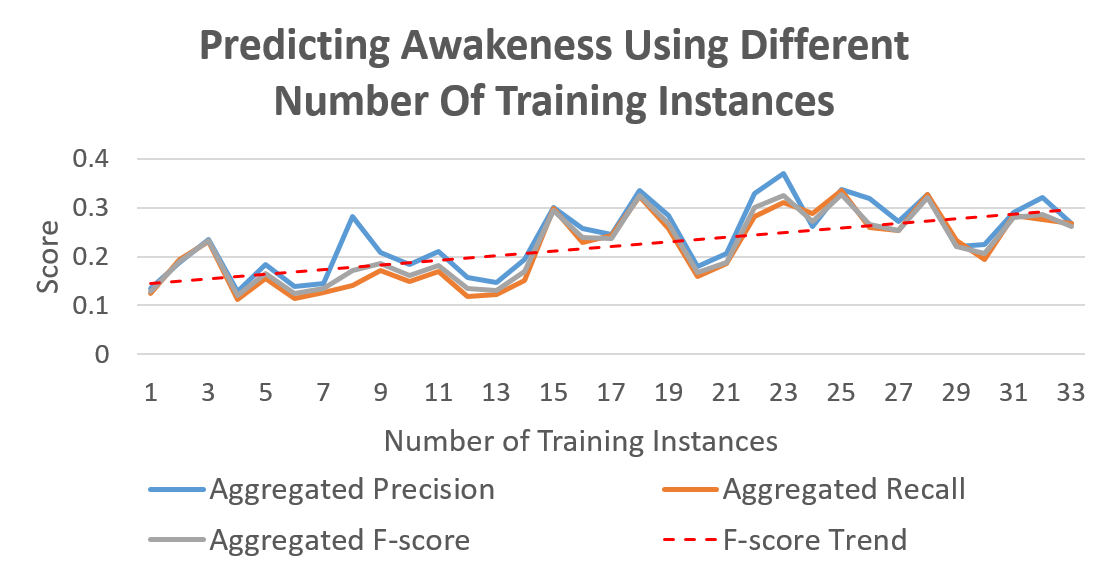
\includegraphics[width=0.5\textwidth]{20180912AwakenessLC2.png}
  \caption{
Performance of the per user trained model measured in precision, recall,
  and f-score. An upwards trending line showing the performance of fscore through the
  different number of training samples is indicated as a dotted red line
  }
   \label{learningCurvet}
\end{figure}

Figure~\ref{learningCurvet} 
shows the performance of a random forest model
trained with the biometric data and predicting the 
left out fold through different numbers training samples.
The data has been binarized as described previously and
the model was trained per each user,
using the survey responses and associated biometric
data of that user. We then evaluated the prediction power for
each of the survey responses of each user, and averaged
the performances for all users.

We show precision, recall, and f-score
to capture the completeness and soundness of our approach 
when predicting the relevant classes, where the relevant
classes are the class for which we have the least number 
of gathered instances (e.g., stressed, not awake, not focused).
This graph shows an overall upwards trend represented by the 
f-score trending line (dotted red) which indicates
that there is a correlation between number of instances trained
on and improvement of the approach's performance.
The trending line shows that there is an improvement of ~9\%
f-score
between training the model with one instance and training
it with 33 instances. Similar results were obtained
when predicting focus and stress.

When contrasting
models trained and tested on the 
biometric data of each user individually, against
a general model trained and tested with the data of all users. 
We can conclude
that for up to 33 training samples analyzed in this study,
the former has better performance when predicting the
responses of each user than when training 
a model with the data of several different users. 
This is partially due to the 
variability across users and the subjective nature
of the responses (e.g.,where slightly awake for one person
may be not awake for another). 

\begin{figure}
  \centering
      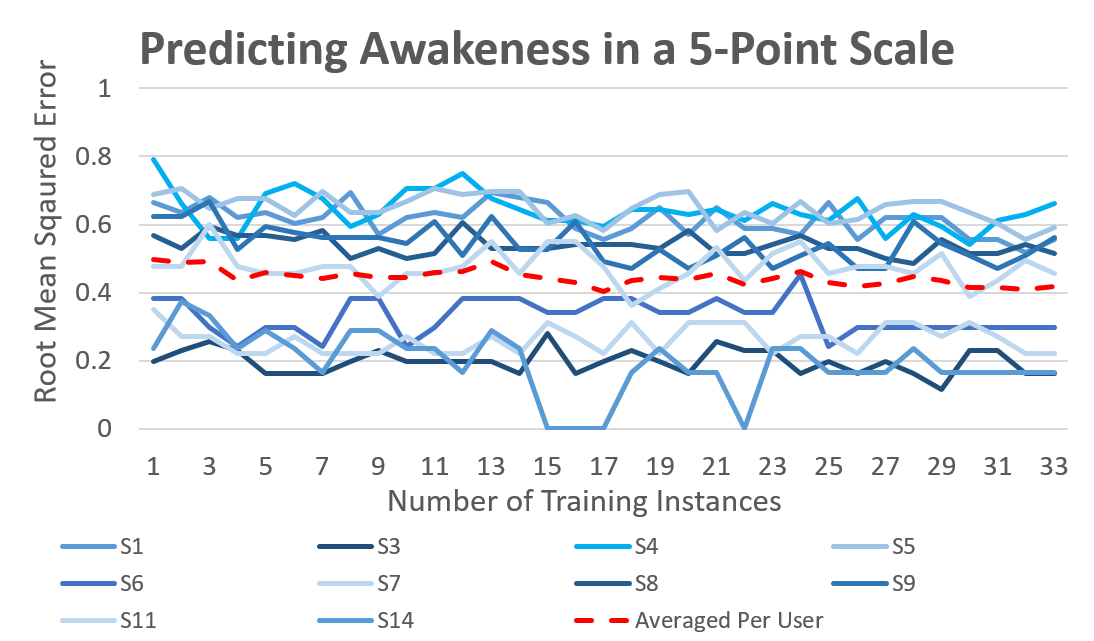
\includegraphics[width=0.5\textwidth]{20180914Awakeness5PointScaleOnly15Lines.png}
  \caption{
Predicting awakeness in a 5-point Likert scale using root mean squared error 
(lower is better)
which indicates how 
  far from the correct answer are the predictions of the model.
  The error decreases as more training instances are added
  }
   \label{learningCurveb}
\end{figure}

Figure~\ref{learningCurveb} 
was created predicting the values in the 5-point
Likert scale, different from binarized responses
as the previous results.
Since the 5-point likert scale is a spectrum
of values and not a binary response, 
the performance of the approach is 
measured using the root mean squared error (lower is better),
which represents how distant is the 
predicted value from the actual value in a 
the scale. 

Figure~\ref{learningCurveb} shows the individual
performance results for each user as straight lines
while the dotted line shows the average of these
performances per user.
The error decreases in an inversely proportional manner
to the number of training samples. The
more training samples add the less likely the 
model will predict a wrong value.
The difference between training with 1 sample (0,49) and training
with 33 samples (0,41) shows a gentle downwards trend in the 
average of all
users.
It is also interesting to notice how the performance results
vary substantially between participants. This means
that for some of the participants the predictions made
by the model are very close most of the time 
to the answer the participant responded
in the survey.

\subsection{Minimum Time Window}
\label{secMinimumTW}
Gathering biometric data is time consuming.
Recognizing which is the minimum time window necessary
to properly predict future responses can make the data
gathering process much faster.
The time windows analyzed refer to the portion of 
time to analyze previous to the start of each survey as 
depicted in Figure~\ref{timeWindows}. These time
windows overlap each with the next (e.g., the 
20 second time window contains all the biometric
data from the 10 second time window, and the
3 hour time window contains the biometric data from
all the previous ones).

\begin{figure}
  \centering
      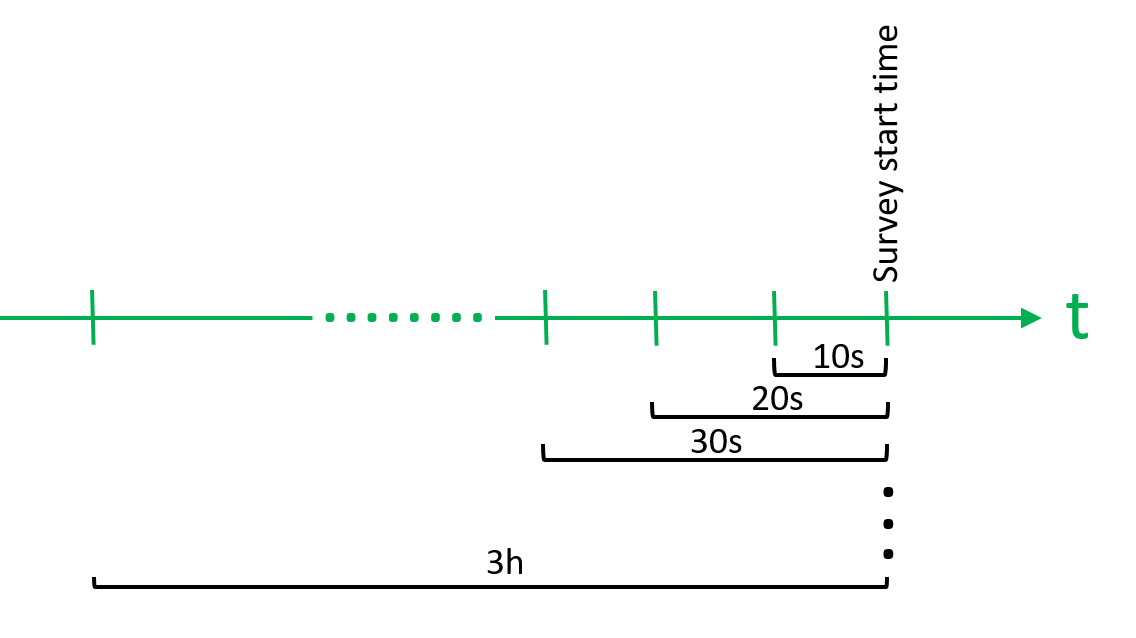
\includegraphics[width=0.4\textwidth]{timeWindows.png}
  \caption{A set of different time windows to gather biometric data previous to each survey response was chosen for analysis. The 16 time windows selected are: 10sec, 20sec, 30sec, 45sec, 1min, 2min, 3min, 5min, 7.5min, 10min, 20min, 30min, 45min, 1hour, 2hour, 3hour}
   \label{timeWindows}
\end{figure}

To determine the optimal time window to analyze biometric
data to predict stress, focus, and awakeness, 
we divided our corpus into the features associated with 
each particular time windows under analysis (16 different
time windows).
We then performed a leave-one-out cross validation
using only the features related to each time window.
Since we are only considering a subset of the features
created for each time window, the 
parameter optimization regarding best number of features 
selected, used in the general model, was
not able to be applied in this section.
We followed the procedure described before by weighting
the model of each user by the number of minority
class instances and aggregating the models' weights
according to their percentage in the overall corpus.

\begin{figure}
  \centering
      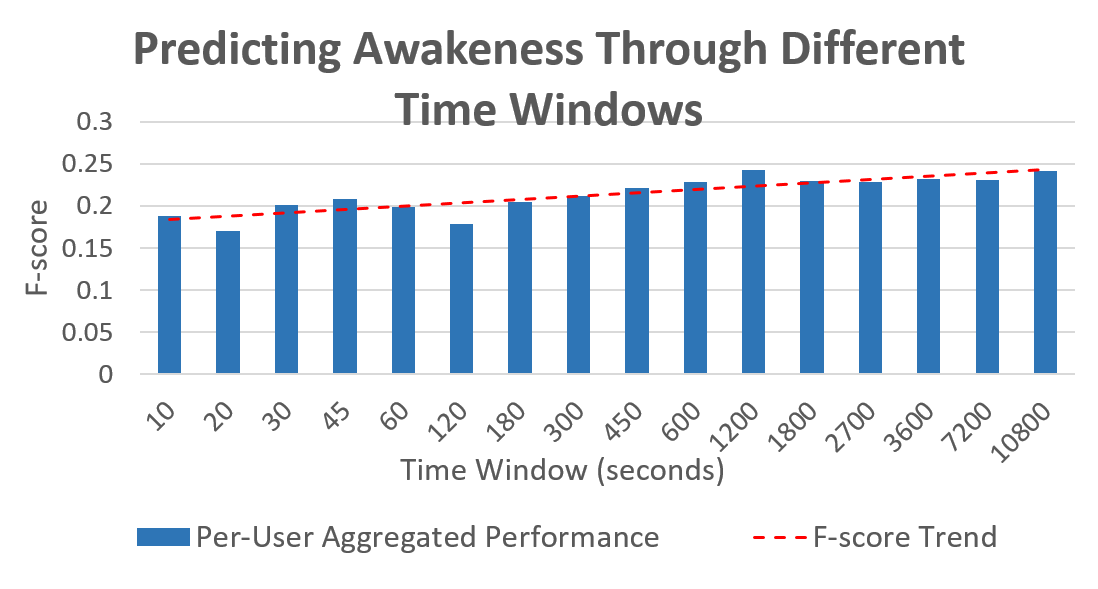
\includegraphics[width=0.5\textwidth]{20180912AwakenessTWBars.png}
  \caption{Performance of a model trained per user predicting
  awakeness using a random forest using different time windows
  }
   \label{timeWindowsPandR}
\end{figure}

Figure~\ref{timeWindowsPandR} shows the precision, recall,
and f-score when predicting awakeness through 16 
different time windows. 
Different from previous analysis where we considered the
full set of features, in this section we consider only the 
features from a single time window. Overall a very
gentle upwards trend is shown with one point
of inflexion in 45 seconds. The performance
through the different time windows stabilizes close 
to 180 seconds.
The best precision, recall, and f-score 
results from the
leave-one-out cross validation are shown in 
the time window corresponding to 10,800 seconds
(3 hours). 

We also compared the performance of a model created per user against
a model created across users.
To calculate the performance of the model created per user,
for each user we create a model using the features 
related to each time window for the selected user only, 
while in the model created with data across users,
we trained the model with the data related to each
particular time window of all users.
our results show that the personalized model created
for each user outperforms in every case
the model created the with data across all users.

This study
shows that in general larger time windows predict stress,
focus, and awakeness more precisely than 
shorter time windows. We can also notice
a very gentle upwards trend
with a inflexion points at 45 seconds and 180.
There is a peak of performance in 45 seconds, 
time window that could be used if time is a scarce resource.
The performance stabilizes around 180 time window
which indicates that collecting data for a longer time
period will not increase significantly the performance of the approach.
The difference in performance between the 
lowest performing and the highest performing time window is 
less than a 10\% improvement. 


\subsection{Computer Interaction Data} \label{secCI}

To collect computer interaction data, we used the open source PersonalAnalytics project\footnote{https://github.com/sealuzh/PersonalAnalytics}  \cite{meyer18} to track participant's mouse and keyboard activity, as well as details about their active window. The specifics of the features tracked are listed in Table \ref{tracker}. The tracker was installed on the computers of 10 of the 14 participants, with participants S6, S10, S12, and S13 opting out of this part of the study. 

\begin{table}
\begin{center}
\begin{tabular}{l l}
\hline

Feature collected by tool& Description \\ 
\hline
Total keystrokes per min& Sum of all types of keystrokes \\ 
Normal keystrokes per min&F[h] Not backspace and navigation \\ 
Backspace keystrokes per min& Backspace keystrokes \\ 
Navigation keystrokes per min& Arrow key keystrokes \\ 
Total clicks per min& Sum of all click types \\ 
Other clicks per min& Not right and left clicks \\ 
Left clicks per min& Left clicks \\ 
Right clicks per min& Right clicks \\ 
Scrolled distance per min& Scrolled distance in pixels \\ 
Moved distance per min& Mouse movements in pixels \\ 
Activity switches per min& Browser window title changes \\ 
Category switches per min& Activity performed category \\ 
\hline
\end{tabular}
\caption{Features collected per user by the computer interaction tracker~\cite{meyer18}}
\label{tracker}
\end{center}
\end{table}

To create the computer interaction features we selected the aforementioned
16 time windows and scaled the values according to the time window. 

We used these computer interaction features to create two new feature sets for each participant: one with only computer interaction features, and one with computer interaction features plus biometric features. Table \ref{ciPerformance} shows the scores that we achieved. We found that in all cases, the computer interaction based model was able to better the results our biometric models. Further, we found that the combined model was the most effective model for predicting stress and awakeness overall, but performed slightly worse than the model using only computer interaction features for focus. Since we consider precision and recall to be the most important statistics when interpreting our results, we compared the models against each other by averaging these two statistics.


\begin{table}
\begin{center}
\begin{tabular}{lllll}
\hline
Model/Feature Set & Accuracy & Precision & Recall\\
\hline
\textbf{Stress}\\
\hspace{3mm}Biometrics only & 0.775 & 0.270 &	0.260\\
\hspace{3mm}C.I. only & 0.698 & 0.290 & 0.272\\
\hspace{3mm}Biometrics + C.I. & 0.712 & 0.317 & 0.286\\
\hline
\textbf{Focus}\\
\hspace{3mm}Biometrics only & 0.716 & 0.251 & 0.256\\
\hspace{3mm}C.I. only & 0.742 & 0.332 & 0.342\\
\hspace{3mm}Biometrics + C.I. & 0.745 & 0.340 & 0.316\\
\hline
\textbf{Awakeness}\\
\hspace{3mm}Biometrics only & 0.808 & 0.269 & 0.314\\
\hspace{3mm}C.I. only & 0.758 & 0.425 & 0.362\\
\hspace{3mm}Biometrics + C.I. & 0.791 & 0.390 & 0.404\\
\hline
\end{tabular}
\caption{A comparison of the results achieved using each of the 3 different feature sets. These values are weighted averages of the individual results from each participant, with more weight given to participants with a larger number of responses. Computer Interactions is abbreviated as C.I. here for readability}
\label{ciPerformance}
\end{center}
\end{table}

As with the biometric models, the individual performance of both the computer interaction only models and the combined models varied quite a bit between participants. Using stress as an example again, in the computer interaction models 5 of the 10 participants saw improvements compared to the baseline, with a maximum improvement of 128\% was seen in precision, and 78\% in recall. In the combined model, referring to stress again, 5 of the 10 participants saw improvements compared to the baseline, with a maximum improvement of 117\% in precision and 95\% in recall. Neither model was capable of correctly predicting any instances of 'stressed' for participant S7.

Since the number of features changes  depending on which feature set is used, we adjusted the feature selection parameter for each of the computer interaction and combined computer interaction/biometric models. The values reported in this section were achieved using the optimal feature selection parameters we found, which are shown in Table \ref{ciFeatureSelection}.

\begin{table}
\begin{center}
\begin{tabular}{lc}
\hline
Model/Feature Set & Number of Features Selected\\
\hline
\textbf{Stress}\\
\hspace{3mm}C.I. & 400\\
\hspace{3mm}Biometrics + C.I. & 800\\
\hline
\textbf{Focus}\\
\hspace{3mm}C.I. & 20\\
\hspace{3mm}Biometrics + C.I. & 300\\
\hline
\textbf{Awakeness}\\
\hspace{3mm}C.I. & All\\
\hspace{3mm}Biometrics + C.I. & 50\\
\hline

\end{tabular}
\caption{The optimal number of features we found to select for each of the model/feature set combinations. Computer interactions is abbreviated as C.I.}
\label{ciFeatureSelection}
\end{center}
\end{table}



